\documentclass[a4paper,11pt]{article}%
    
\usepackage{fullpage}%
\usepackage[T1]{fontenc}%
\usepackage[utf8]{inputenc}%


\usepackage[french]{babel}% % Adjust the main language


\usepackage{graphicx}%
\usepackage{url}%
\usepackage{abstract}%
\usepackage{lipsum}
\usepackage{mathpazo}%
\usepackage{multicol}
\usepackage{listings}%
\usepackage[linesnumbered,ruled,vlined]{algorithm2e}
\usepackage{subcaption}
\usepackage{xcolor}

\parskip=0.5\baselineskip

\sloppy

\begin{document}

\title{Création d'une \emph{Learning Heuristic} pour résoudre le \emph{Capacitated Vehicle Routing Problem}}

\author{Clément Legrand-Lixon}

\maketitle

\begin{abstract}
Les problèmes d'optimisation sont des problèmes difficiles à résoudre de manière exacte. 
Le \emph{Capacitated Routing Vehicle Problem} est l'un de ces problèmes, et est très étudié dans la littérature. 
Pour approcher les solutions optimales, différents types d'algorithme existent.
Des méthodes d'extraction de connaissance voient le jour afin d'améliorer les performances d'algorithme existant. 

\end{abstract}

\section*{Introduction}
Le Vehicle Routing Problem (VRP), consiste à relier un nombre $n$ de clients par des tournées, commençant et finissant toutes à un même point défini, le dépôt. 
Ce problème est NP-complet, et dispose de nombreuses applications dans le monde d'aujourd'hui (notamment gestion d'un réseau routier). 
D'autant plus que ce problème dispose de nombreuses variantes (ajout d'une contrainte de temps, plusieurs dépôts possibles...). 
L'une des variantes les plus connues consiste à prendre en compte pour chaque client sa demande, de sorte à ce que les tournées créées ne dépassent pas une certaine capacité définie à l'avance. 
On nomme ce problème Capacitated Vehicle Routing Problem (CVRP). 

Si de nombreuses heuristiques ont vu le jour pour résoudre ce problème, aucune d'entre elles ne parvient à trouver des solutions optimales pour toutes les instances de la littérature, malgré de très bons résultats dans la plupart des cas. Récemment~\cite{Sorensen_2017}, une nouvelle heuristique efficace a vu le jour. L'objectif de mon stage est de créer une \emph{Learning Heuristic} afin de trouver de meilleures solutions.

Ce rapport commence par présenter le problème étudié, et introduit les notations et opérateurs utilisés dans la suite. Il présente ensuite l'objectif du stage et la méthode mise en place pour y parvenir. 
Différents problèmes sont alors soulevés, et sont traités dans chacune des parties qui suit.
  

\section{Présentation des notions et notations}
Cette partie introduit le problème étudié ainsi que les différentes notations utilisées ensuite dans le reste du rapport. 

\subsection{Optimisation combinatoire}
Un problème d'optimisation combinatoire (également appelée optimisation discrète), consiste à   trouver dans un ensemble discret les meilleures solutions réalisables. 
La notion de meilleure solution étant définie par une fonction objectif.
Formellement, on a :
\begin{itemize}
\item Un ensemble discret $N$;
\item Une fonction $f : 2^N \rightarrow \Re$, dite fonction objectif;
\item Un ensemble $R$ de sous-ensembles de $N$, dont les éléments sont appelés solutions réalisables.
\end{itemize}
Ainsi, un problème d'optimisation combinatoire consiste à déterminer :

\begin{center}
$ max_{S \subseteq N} \{ f(S), S \in R \} $
\end{center}

Beaucoup trop de solutions

\subsection{Description du problème}
Le problème étudié ici (CVRP) est une extension du problème (VRP). Ces problèmes font partie de la famille des problèmes d'optimisation stochastique.

\subsubsection{Problèmes d'optimisations}

\subsubsection{Vehicle Routing Problem (VRP)}

Le problème de tournées de véhicules, est un problème NP-complet, où sont donnés $n$ points de coordonnées $(x_i,y_i)$, représentant 1 dépôt et $n-1$ clients. $k$ véhicules sont disponibles. 
L'objectif est alors de minimiser la longueur du réseau (ensemble des tournées). 
On définit alors $x_{i,j}^v$ qui vaut 1 si $j$ est desservi après $i$ par le véhicule $v$, et 0 sinon. 
On définit également $c_{i,j}$ comme étant la distance entre $i$ et $j$.
Il faut donc déterminer la solution $Sol$ vérifiant :
\begin{center}
$ Sol = argmin_{Sol} \sum_{i = 0}^{n} \sum_{j = 0}^{n} \sum_{v = 1}^{k} c_{i,j} x_{i,j}^v = argmin_{Sol}cost(Sol)$
\end{center}

Les tournées créées doivent également respecter les contraintes suivantes :
\begin{itemize}
\item Chaque client doit être desservi par une et une seule tournée;
\item Chaque tournée doit partir et s'arrêter au dépôt.
\end{itemize}

Un exemple d'instance est présenté en figure~\ref{Instance3205}, où les points rouges représentent les clients et le point bleu le dépôt. Une solution possible au problème est représenté en figure~\ref{SNC3205} mais n'est à priori pas optimale. 
De nombreux algorithmes ont vu le jour pour tenter de résoudre ce problème, ainsi que les nombreuses variantes qui existent (ajout de contraintes de capacité, temps ou longueur sur les tournées, ces contraintes sont cumulables). 
C'est l'ajout de capacité aux tournées qui nous intéressera plus particulièrement.


\begin{figure}

\centering
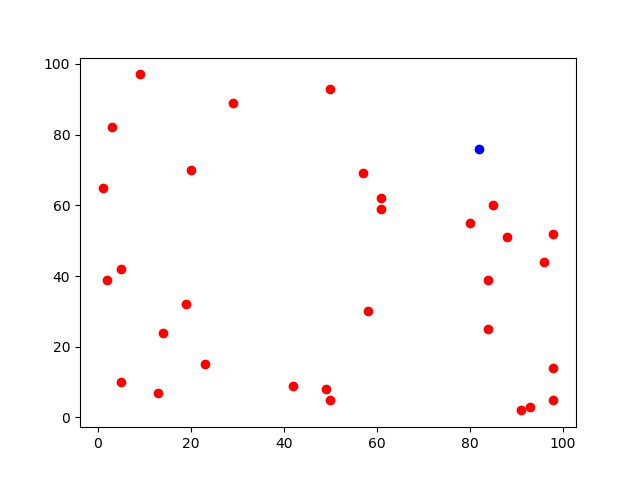
\includegraphics[scale=0.5]{Instance.png}
\caption{Représentation de l'instance A-n32-k05 de la littérature}
\label{Instance3205}
\end{figure}

\begin{figure}

\centering
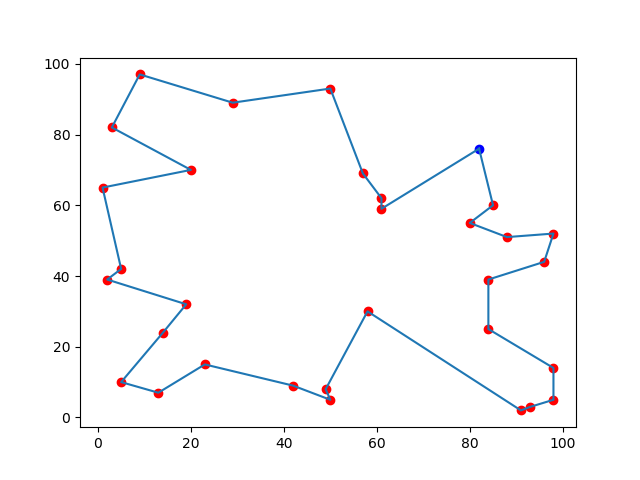
\includegraphics[scale=0.5]{solutionNoCapacity.png}
\caption{Représentation d'une solution de l'instance A-n32-k05}
\label{SNC3205}
\end{figure}

\subsubsection{Capacitated VRP (CVRP)}

On étend le VRP au CVRP en ajoutant à chaque client $i$ une demande $d_i$, ainsi qu'une capacité $C$ aux véhicules.
Une nouvelle contrainte vient donc s'ajouter aux contraintes classiques du VRP :
\begin{itemize}
\item La demande totale sur chaque tournée ne doit pas excéder la capacité du véhicule.
\end{itemize}
Si on reprend l'instance A-n32-k05, en considérant les demandes des clients ainsi que la capacité disponible pour chaque véhicule, on obtient une solution présente sur la figure~\ref{SC3205}, qui n'est pas optimale. 
Ce problème est beaucoup étudié car il a de nombreuses applications (comme par exemple la gestion du trafic routier, ou alors la gestion d'un réseau de bus), et peu de solutions optimales ont été trouvées pour des instances de plus de $500$ clients. 

\begin{figure}
\centering
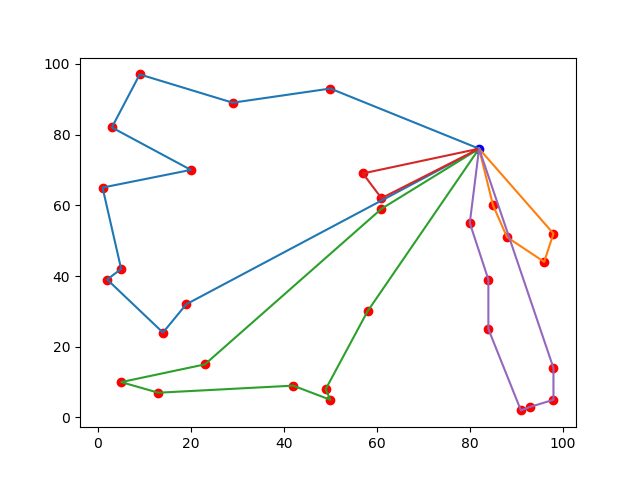
\includegraphics[scale=0.5]{solutionCapacity.png}
\caption{Représentation d'une solution de l'instance A-n32-k05, où les demandes des clients sont prises en compte}
\label{SC3205}
\end{figure}

\subsection{Parcours et exploration des voisinages}
\label{voisinage}

Lorsqu'il s'agit de trouver une solution optimale à un problème, il est souvent intéressant d'explorer les voisinages d'une solution pour voir s'il n'y a pas mieux. Selon la méthode d'exploration employée, il peut être intéressant de parcourir le voisinage de différentes manières, pour ne pas toujours favoriser les mêmes voisins.

L'\underline{exploration} d'un voisinage de solutions peut être plus ou moins exhaustif selon la condition d'arrêt utilisée.
On distingue principalement, deux conditions d'arrêt lorsqu'il s'agit d'explorer des voisinages :

\begin{itemize}
\item First improvement (\emph{FI}) : on parcourt le voisinage jusqu'à trouver un changement qui améliore la solution actuelle (on s'arrête donc à la première amélioration trouvée);
\item Best improvement (\emph{BI}) : on parcourt tout le voisinage, et on applique le changement qui va le plus améliorer notre solution actuelle. \\
\end{itemize}

Pour explorer un voisinage, on peut le \underline{parcourir} de différentes manières de sorte à ne pas toujours favoriser les mêmes voisins. On considérera ici 3 parcours différents : 

\begin{itemize}
\item Dans l'ordre (\emph{O}) : les voisins sont parcourus dans un ordre naturel (du premier au dernier);
\item Dans un semi-ordre (\emph{SO}) : on commence le parcours là où on s'était arrêté au dernier parcours, on parcourt ensuite les voisins dans l'ordre;
\item Aléatoirement (\emph{RD}) : on tire aléatoirement l'ordre dans lequel on va parcourir les voisins. \\
\end{itemize}

On peut remarquer que peu importe le parcours effectué, pour faire une exploration \emph{BI}, il faudra passer par tous les voisins. Pour qu'une exploration \emph{FI} soit efficace, il faut éviter un parcours \emph{O}, car dans ce cas on privilégie une certains voisinages qui seront choisis plus souvent. On retiendra le tableau récapitulatif suivant:

\begin{center}
\begin{tabular}{|c|c|c|}
   \hline
     & \emph{BI} & \emph{FI}  \\
   \hline
   \emph{O} & Oui & Non \\
   \hline
   \emph{SO} & Non & Oui \\
   \hline
   \emph{RD} & Non & Oui  \\
   \hline
\end{tabular}
\end{center}


\subsection{Motivation et objectif}

L'objectif de mon stage d'intégrer de la connaissance à un algorithme d'optimisation utilisé pour résoudre CVRP, afin de le rendre plus performant.
Une idée pour y parvenir serait de réussir à prédire des arêtes qui appartiendront à la solution optimale, en n'observant que des solutions initiales que l'on peut générer rapidement. 
On pourra ensuite exploiter ces arêtes pour construire une nouvelle solution.
Nous adopterons la méthodologie suivante pour atteindre notre objectif :
\begin{itemize}
\item Comparer des solutions initiales à des solutions optimales pour des petites instances;
\item Établir de l'étude précédente des règles qui permettent de caractériser ces arêtes;
\item Exploiter les arêtes obtenues dans un algorithme d'optimisation.
\end{itemize}

Cette méthode, nous impose de résoudre les problèmes suivants : Comment construire une solution initiale de bonne qualité ? Quel algorithme d'optimisation utiliser ? Comment extraire la connaissance ? Comment intégrer la connaissance dans l'algorithme d'optimisation retenu ?

\section{Construction d'une solution initiale de bonne qualité}
\label{SolInit}
Pour construire une solution initiale nous allons utiliser la dernière version d'un algorithme très répandu dans la littérature : l'algorithme Clarke \& Wright~\cite{Altinel_2005}.

\subsection{Description de l'algorithme}
L'algorithme Clarke \& Wright (CW) est un algorithme glouton. 
Initialement chaque client est desservi par un véhicule (de cette manière la contrainte sur le nombre de véhicules disponibles n'est pas respectée). Ensuite les tournées sont fusionnées en fonction des \emph{savings} calculées.
On définit le \emph{saving} des clients $i$ et $j$ de la manière suivante :

\begin{center}
$s(i,j) = c_{i0} + c_{0j} - \lambda c_{ij} + \mu \vert c_{i0} - c_{0j} \vert + \nu \frac{d_i + d_j}{\overline{d}}$
\end{center}

Les paramètres $(\lambda, \mu, \nu)$ jouent un rôle important dans la formule précédente, ce que nous verrons plus tard. (rôle des paramètres à détailler). 

L'algorithme \ref{algo:CW} présente le fonctionnement de l'algorithme CW.

\begin{algorithm}
\DontPrintSemicolon % Some LaTeX compilers require you to use \dontprintsemicolon instead
\KwIn{Un ensemble de points I, un ensemble d'entiers $D = {d_1,...,d_n}$ et un triplet $(\lambda,\mu,\nu)$ de flottants}
\KwOut{Une solution au problème I}

\For{$i \gets 1$ \textbf{to} $n$} {
	$Sol \gets Sol \cup [0,i,0]$\;
}
Calculer les savings de toutes les arêtes\;

\While {max$_{i,j} s(i,j) > 0$} {
	$(i,j) \gets argmax_{(i,j)} s(i,j)$\;
	$r_i \gets findRoute(Sol,i)$\;
	$r_j \gets findRoute(Sol,j)$\;
	\If{$r_i$ et $r_j$ peuvent fusionner} {
		Retirer $r_i$ et $r_j$ de $Sol$\;
		Si possible fusionner $r_i$ et $r_j$\;
		Ajouter le résultat dans $Sol$ et mettre $s(i,j) = 0$\;
	}
}

\Return{$Sol$}\;
\caption{{\sc Clarke-Wright} calcule une solution initiale}
\label{algo:CW}
\end{algorithm}

Exemple d'exécution de l'algorithme avec $(\lambda, \mu, \nu) = (1,1,1)$, sur l'instance A-n37-k06, représenté sur les figures \ref{CWinit} à \ref{resCW101010}. On remarque sur la figure \ref{resCW101010} que l'on pourrait améliorer la solution rien qu'en réorganisant les différentes tournées, pour minimiser leur coût.

\begin{figure}
\begin{center}




  	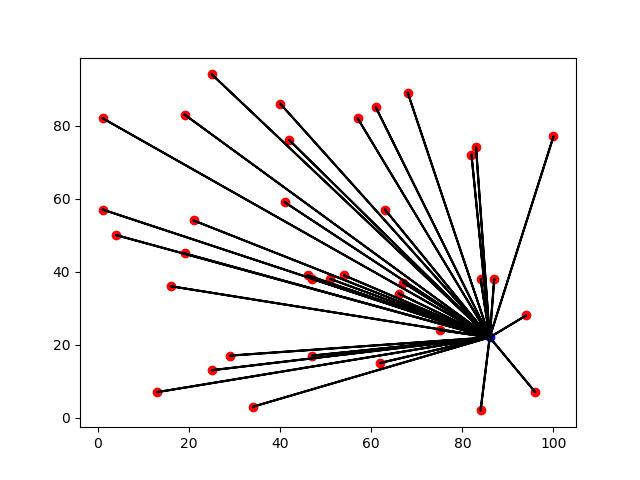
\includegraphics[scale=0.4]{CWinit.png}
  	\caption{Initialisation}
	\label{CWinit}
	
  
  
	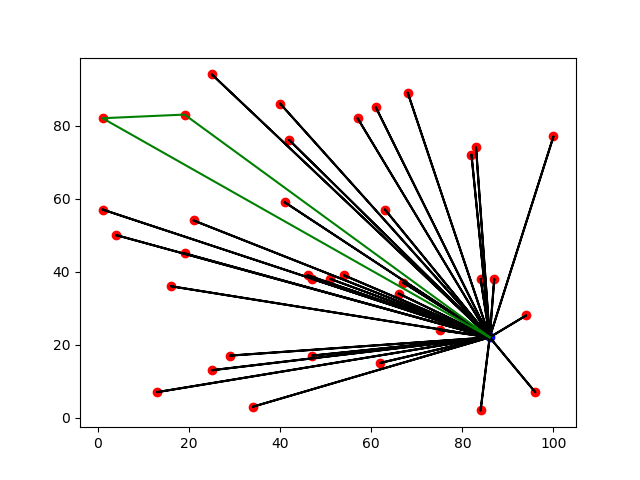
\includegraphics[scale=0.4]{CW1.png}
	\caption{1$^{ere}$ fusion}
 	\label{CW1}
  	


	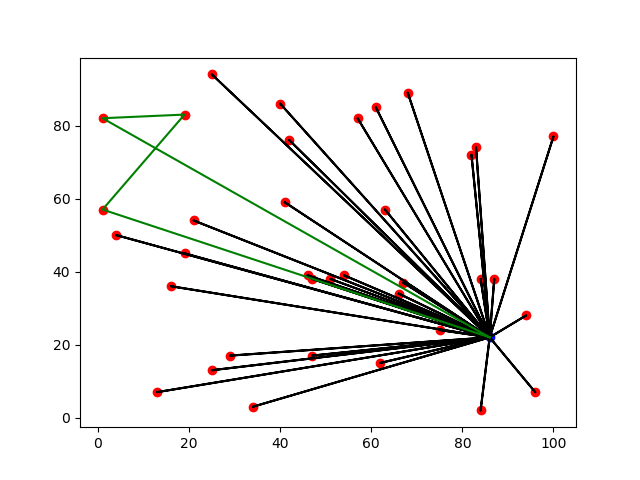
\includegraphics[scale=0.4]{CW2.png}
	\caption{2$^{eme}$ fusion}
	\label{CW2}


	 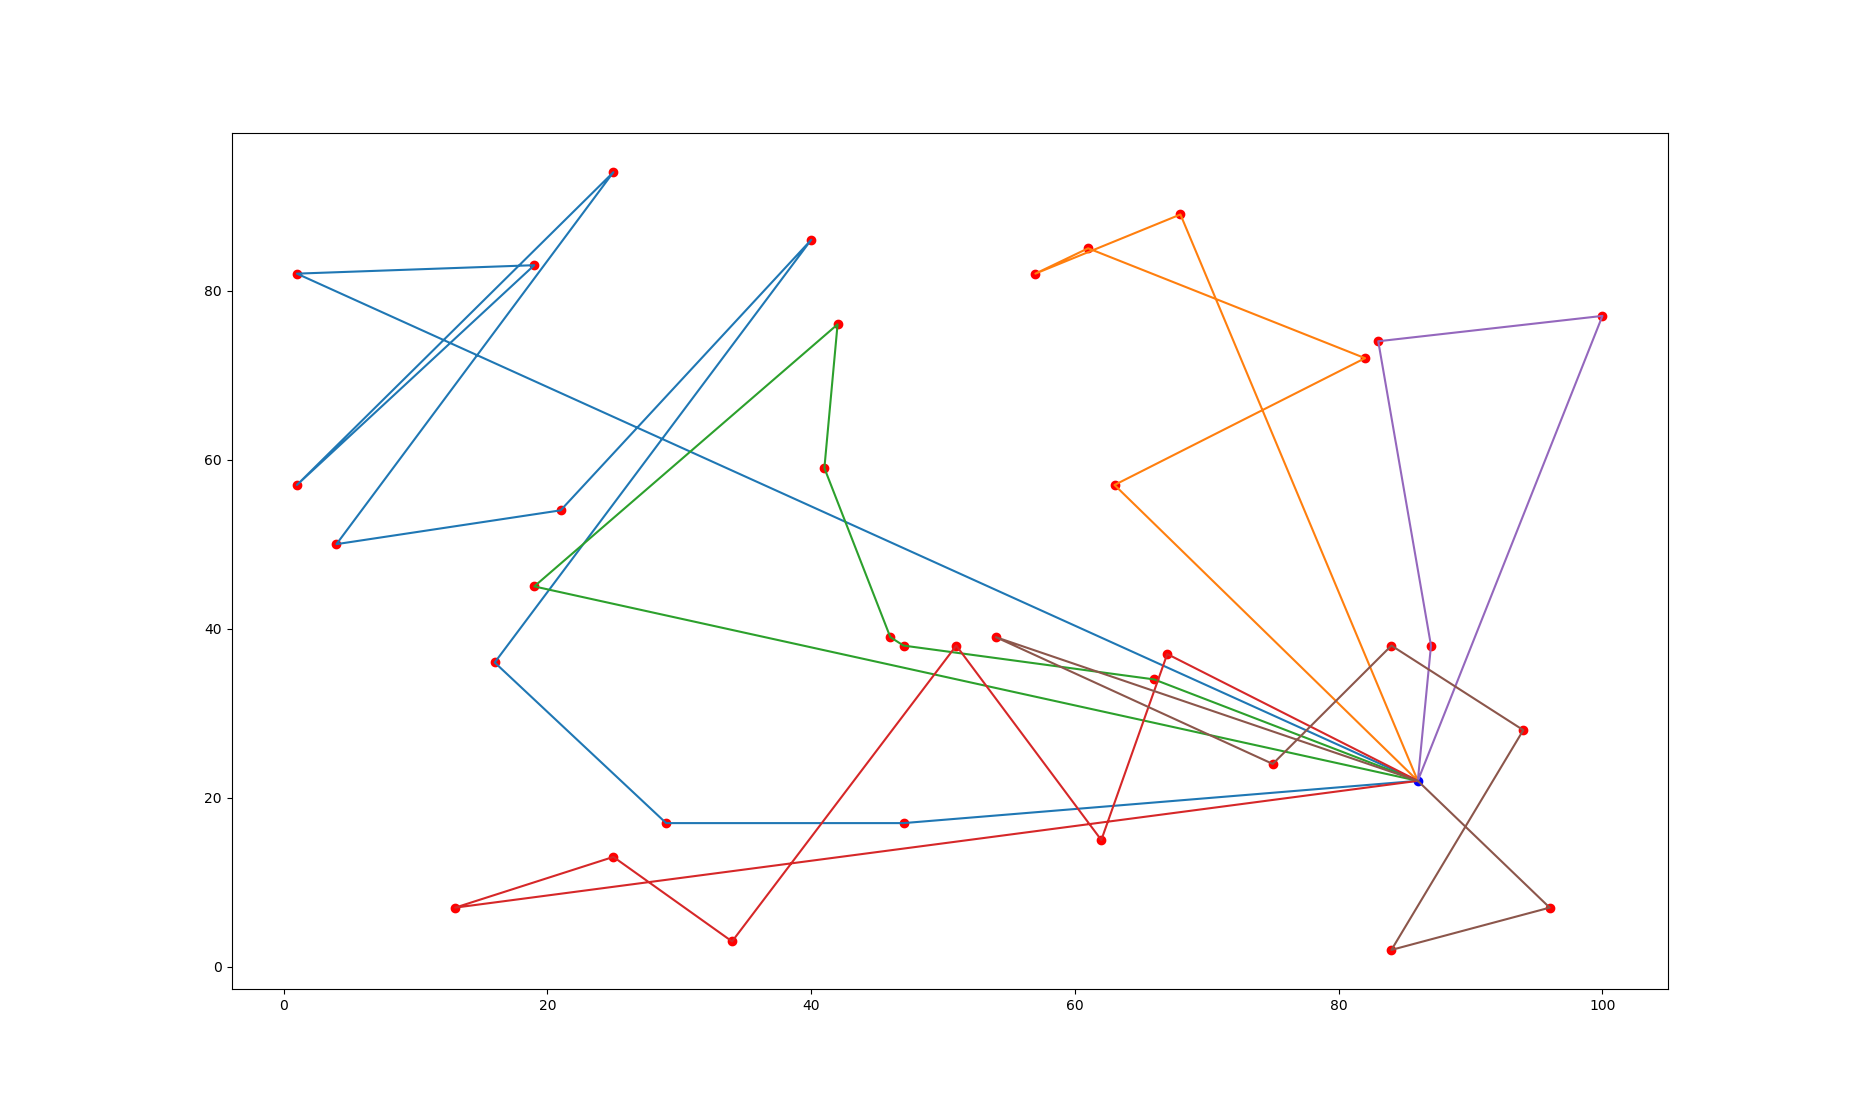
\includegraphics[scale=0.15]{resCW101010.png}
	 \caption{Solution obtenue, $cost = 1297$}
	\label{resCW101010}

\end{center}
\end{figure}


 
\subsection{Choix des paramètres $(\lambda, \mu, \nu)$}
Le triplet $(\lambda, \mu, \nu)$ a déjà été étudié de nombreuses fois dans la littérature. L'article~\cite{Altinel_2005} précise qu'il suffit de considérer $(\lambda, \mu, \nu)$ dans $]0,2] \times [0,2]^2$ pour avoir de bonnes solutions. 
Par ailleurs, il est inutile de prendre précision inférieure au dixième lorsqu'on choisit les valeurs des paramètres.
Les figures \ref{resCW190105} à \ref{resCW001015} représentent différents résultats obtenus pour des triplets $(\lambda, \mu, \nu)$ différents.
On remarque qu'il n'y a aucun lien entre les résultats et les valeurs de $(\lambda, \mu, \nu)$. 
On ne peut donc pas prévoir à l'avance si le triplet $(\lambda, \mu, \nu)$ va donner un bon résultat ou non. 
L'influence de ces paramètres dépend aussi des caractéristiques de l'instance considérée, ainsi on ne peut pas se restreindre au choix d'un triplet qui conviendrait pour toutes les instances. 


\begin{figure}
\begin{center}

	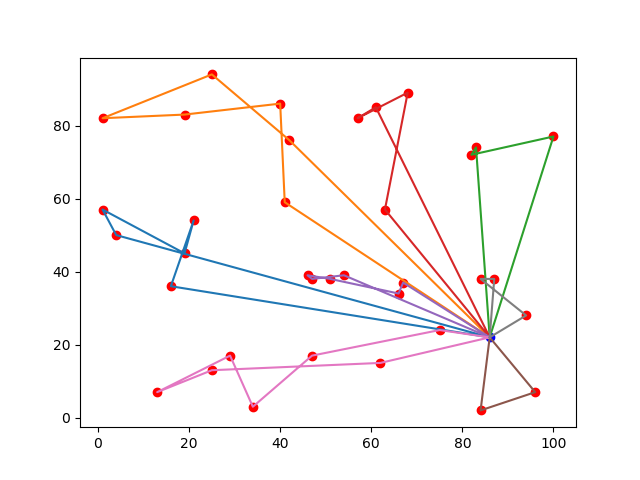
\includegraphics[scale=0.4]{resCW190105.png}
 
 	\caption{$(1.9,0.1,1.5), cost = 1106$}
 	\label{resCW190105}

	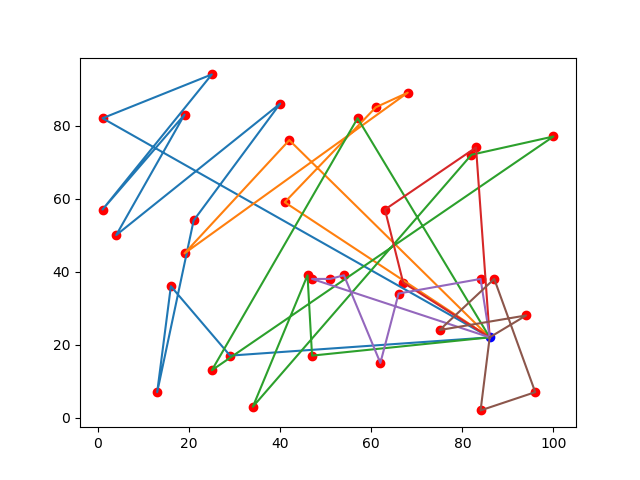
\includegraphics[scale=0.4]{resCW111.png}
	
	\caption{$(0.1,0.1,0.1), cost = 1569$}
	\label{resCW111}

	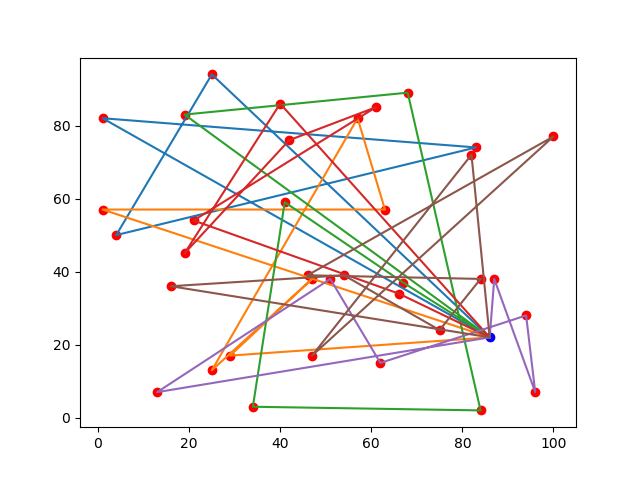
\includegraphics[scale=0.4]{resCW001015.png}
 	\caption{$(0.0,1.0,1.5), cost = 2191$}
 	\label{resCW001015}
\end{center}
\end{figure}

\section{Proposition d'un algorithme d'optimisation}
Nous proposons dans cette partie un algorithme d'optimisation qui sera utilisé pour y intégrer de la connaissance. Il s'inspire d'un algorithme proposé récemment~\cite{Sorensen_2017}, dont nous détaillons le fonctionnement.

\subsection{Heuristique Arnold \& Sörensen}
L'heuristique proposée par Arnold et Sörensen, est à la fois simple et efficace. 
Il semble donc pertinent de vouloir améliorer cet algorithme en y intégrant de la connaissance.
L'heuristique commence par déterminer une solution initiale via l'algorithme CW, présenté en section~\ref{SolInit}. Différents opérateurs de voisinage sont ensuite appliqués autour d'une arête, considérée comme étant la pire du graphe.
L'algorithme~\ref{algo:AS} donne le fonctionnement de l'heuristique (A\&S). 


\begin{algorithm}
\DontPrintSemicolon % Some LaTeX compilers require you to use \dontprintsemicolon instead
\KwIn{Un ensemble de points I, les demandes des clients D, un triplet de flottants $(\lambda,\mu,\nu)$}
\KwOut{Une solution au problème I}
$Sol \gets CW(I,D,\lambda,\mu,\nu)$\;
$N \gets Size(D)$\;
$nextSol \gets Sol$\;
\While {La dernière amélioration date de moins de 3 min} {
	$worstEdge \gets$ Calcul de la pire arête\;
	$nextSol \gets EC_{BI-O}(worstEdge,I,D)$\;
	$nextSol \gets LK_{BI-O}(nextSol)$\;
	$nextSol \gets CE_{BI-O}(worstEdge,I,D)$\;
	$nextSol \gets LK_{BI-O}(nextSol)$\;
	\If {$cost(Sol) > cost (nextSol)$} {
		$ Sol \gets nextSol$\;
	}
	\If {Pas d'améliorations depuis $N/10$ itérations} {
		Appliquer les opérateurs sur toutes les arêtes de la solution\;
	}
	\If {Pas d'améliorations depuis $20N$ itérations} {
		Changer de fonction de pénalisation en prenant un autre triplet $(\gamma_w,\gamma_c,\gamma_d)$\;
	}
	\If {Pas d'améliorations depuis $100N$ itérations} {
		Réinitialiser les pénalités des arêtes\;
	}
}
\Return{$Sol$}\;
\caption{{\sc AS} applique l'heuristique A\& S au problème considéré}
\label{algo:AS}
\end{algorithm}

Les prochaines sections détaillent le calcul de la pire arête, ainsi que le fonctionnement des opérateurs utilisés.


\subsubsection{Pire arête et pénalisation}
Afin de pouvoir comparer les différentes arêtes entre elles et déterminer laquelle est la pire, il faut disposer de certaines métriques sur les arêtes pour pouvoir les caractériser.

Trois métriques sont détaillées dans l'article~\cite{Sorensen_2017}:
\begin{itemize}
\item Le coût d'une arête $(i,j)$, que l'on note $c(i,j)$ se calcule de la manière suivante:

\begin{center}
$c(i,j) = c_{ij}(1 + \beta p(i,j)$ 
\end{center}

Dans l'article~\cite{Sorensen_2017}) $\lambda = 0.1$. $p(i,j)$ correspond au nombre de fois où l'arête $(i,j)$ a été pénalisé;
\item La profondeur d'une arête $(i,j)$, noté $d(i,j)$ a pour formule :

\begin{center}
max($c_{0i}$, $c_{0j}$)
\end{center}

Autrement dit c'est la distance entre le point le plus éloigné du dépôt et le dépôt.
\item La largeur de l'arête $(i,j)$, noté $w(i,j)$ est la différence de longueur entre les projetés de $i$ et $j$ sur la droite issue du dépôt passant par le centre de gravité de la tournée. Le centre de gravité d'une tournée étant obtenu en faisant la moyenne, pour chaque composante, des points de cette tournée.
\end{itemize}

Les notions de coût, profondeur et largeur sont illustrées par la figure~\ref{metrics}. 

\begin{figure}
\centering
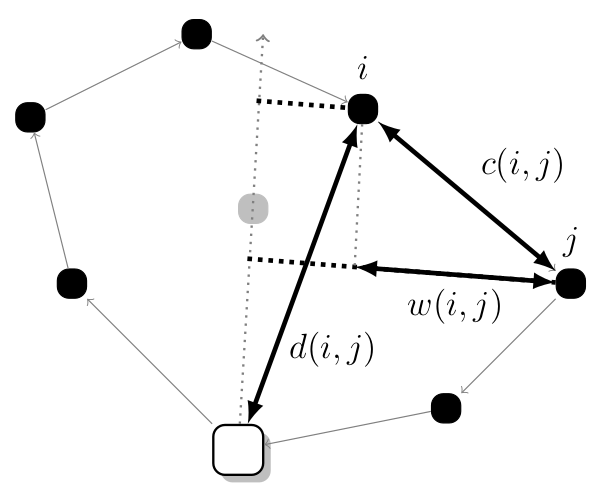
\includegraphics[scale=0.3]{metrics_big.png}
\caption{Illustration des caractéristiques d'une arête}
\label{metrics}
\end{figure}

On définit alors la fonction de pénalisation $b$ de la manière suivante :
\begin{center}
$b(i,j) = \frac{[\gamma_w w(i,j) + \gamma_c c(i,j)] [\frac{d(i,j)}{max_{k,l}d(k,l)}] ^ {\frac{\gamma_d}{2}}}{1+p(i,j)}$
\end{center}

Les paramètres $\lambda_w,\lambda_c,\lambda_d$, prennent comme valeurs $0$ ou $1$, selon les caractéristiques que l'on veut considérer. 
Il y a ainsi 6 fonctions de pénalisation différentes, que l'on peut choisir au cours de l'exécution (on ne considère pas le cas où $\lambda_w = \lambda_c = 0$, puisqu'il fournit $b(i,j) = 0$.

On peut alors définir ce qu'est la pire arête $(i^*,j^*)$ du graphe :

\begin{center}
$ (i^*,j^*) = argmax_{i,j} b(i,j)$
\end{center}



C'est autour de l'arête calculée ici que vont s'orienter les recherches des opérateurs de voisinage qui suivent.
 
\subsubsection{Ejection-Chain}

Le premier opérateur utilisé est appelé Ejection-Chain. Son objectif est de déplacer au plus $l$ clients sur des tournées. 

Le fonctionnement de cet opérateur est présenté sur la figure~\ref{EC}.

\begin{figure}
\centering
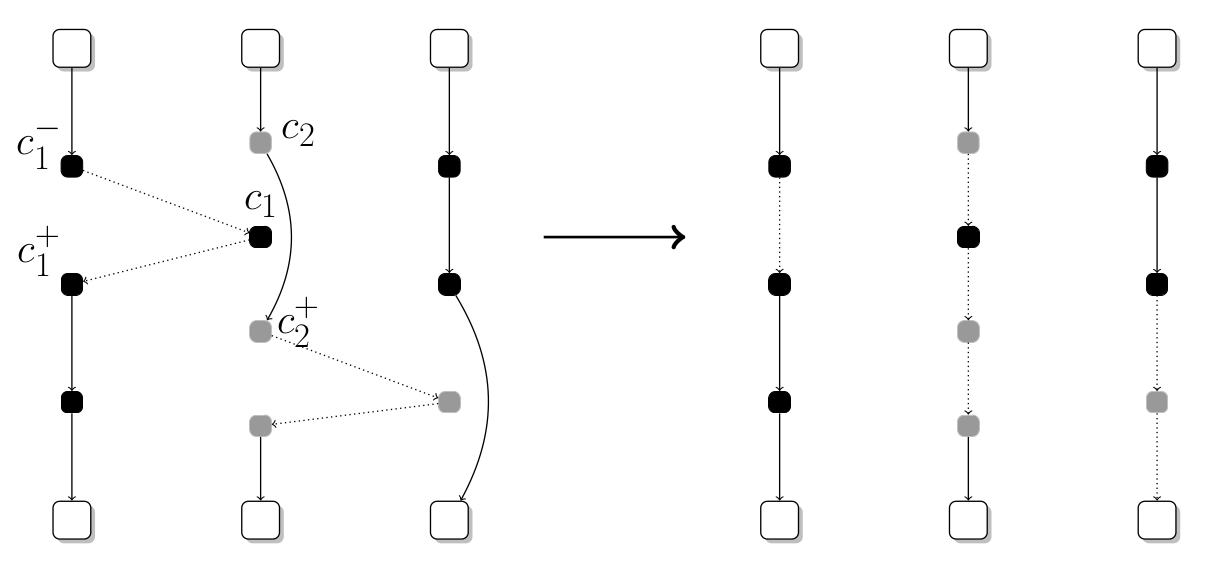
\includegraphics[scale=0.2]{ejection_chain_big.png}
\caption{Exemple de fonctionnement de l'opérateur ejection-chain}
\label{EC}
\end{figure}

Dans l'article~\cite{Sorensen_2017} $l = 3$. En effet l'algorithme~\ref{algo:EC}, qui décrit le fonctionnement de cet opérateur, s'exécute en $O(n^{l-1})$. Il vaut donc mieux choisir une valeur de $l$ assez petite, pour que la complexité n'explose pas. 

\begin{algorithm}
\DontPrintSemicolon % Some LaTeX compilers require you to use \dontprintsemicolon instead
\KwIn{Une arête $(a,b)$, la liste des plus proches voisins des clients $voisins$, un entier $l$, la solution actuelle $sol$}
\KwOut{Une nouvelle solution au moins aussi bonne que $sol$}
$possibleSol \gets sol$\;
$cand \gets choose(a,b)$\;
$nextRoute \gets findNextRoute(cand,voisins,possibleSol)$\;
$possibleSol \gets $ déplacer $cand$ après son voisin sur $nextRoute$\;
\For{$i \gets 1$ \textbf{to} $l-1$} {
  $cand \gets $un client de $nextRoute$ différent de celui ajouté\;
  $nextRoute \gets findNextRoute(cand,voisins,possibleSol)$\;
  $possibleSol \gets$ déplacer $cand$ après son voisin sur $nextRoute$\;
}
\If {$cost(possibleSol) < cost(sol)$} {
	$sol \gets possibleSol$\;
}
\Return{$sol$}\;
\caption{{\sc Ejection-Chain} applique l'opérateur ejection-chain}
\label{algo:EC}
\end{algorithm}

Aux lignes $3, 4, 7$ et $8$ de l'algorithme~\ref{algo:EC}, il est possible d'utiliser les méthodes de la section~\ref{voisinage} pour explorer les voisinages.

\subsubsection{Cross-Exchange}

Un deuxième opérateur utilisé est le Cross-Exchange.
Son objectif est d'échanger deux séquences de clients entre deux tournées.
Le fonctionnement de cet opérateur est présenté sur la figure~\ref{CE}.

\begin{figure}
\centering
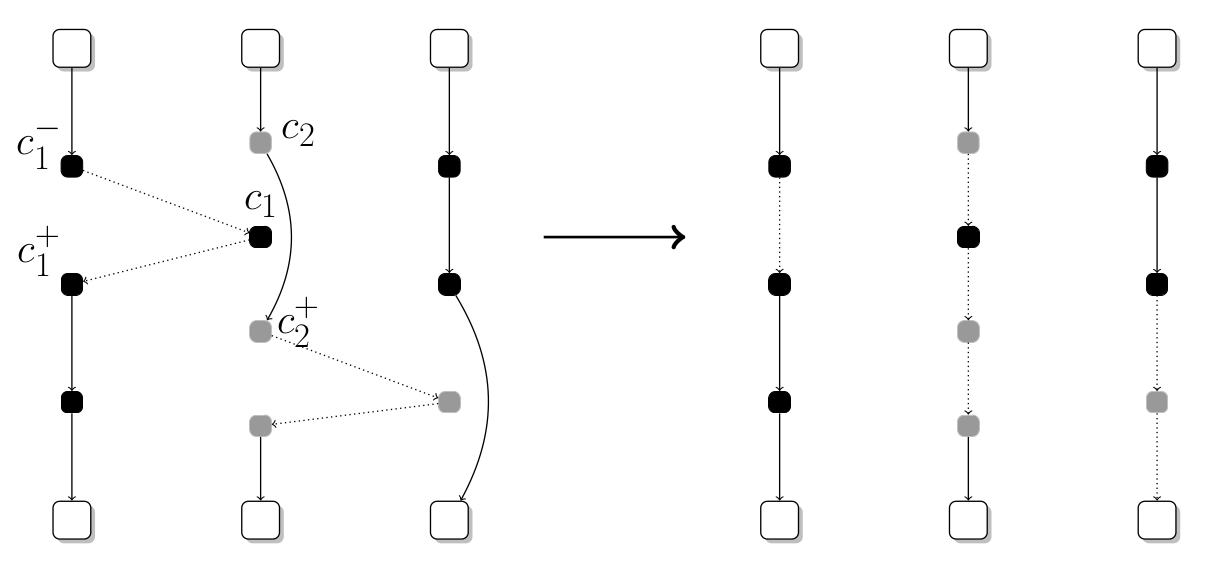
\includegraphics[scale=0.2]{cross_exchange_big.png}
\caption{Exemple de fonctionnement de l'opérateur cross-exchange}
\label{CE}
\end{figure}

Il est possible de limiter le nombre de clients par séquence échangée.
L'algorithme~\ref{algo:CE} présente l'exécution de l'opérateur et s'exécute en $O(n^2)$.

\begin{algorithm}
\DontPrintSemicolon 
\KwIn{Une arête $(c_1,c_2)$, la liste des plus proches voisins des clients $voisins$, la solution actuelle $sol$}
\KwOut{Une nouvelle solution au moins aussi bonne que $sol$}
$possibleSol \gets sol$\;
$nextRoute \gets findNextRoute(c_1,voisins,possibleSol)$\;
Considérer l'arête $(c_3,c_4)$ de $nextRoute$, où $c_4$ est le proche voisin de $c_1$ utilisé\;
$possibleSol \gets exchange(c_1,c_3,possibleSol)$\;
Choisir 2 clients $c_5$ et $c_6$ qui n'appartiennent pas à la même tournée\;
$possibleSol \gets exchange(c_5,c_6,possibleSol)$\;
\If {$cost(possibleSol) < cost(sol)$} {
	$sol \gets possibleSol$\;
}
\Return{$sol$}\;
\caption{{\sc Cross-Exchange} applique l'opérateur cross-exchange}
\label{algo:CE}
\end{algorithm}

A la ligne $6$ de l'algorithme~\ref{algo:CE}, il est possible d'utiliser les méthodes de la section \ref{voisinage} pour explorer les voisinages, et choisir les clients à échanger.

\subsubsection{Lin-Kernighan}

Le dernier opérateur utilisé est l'heuristique Lin-Kernighan. Elle a été créée pour résoudre le problème du voyageur de commerce (TSP). 
Il effectue une optimisation intra-tournée (c'est-à-dire que la tournée considérée est améliorée indépendamment des autres).
Cela consiste en une réorganisation des clients sur la tournée. On choisit $k$ tel que \emph{LK} ne dépasse pas \emph{k-opt} au cours de son exécution. 
On appelle \emph{k-opt}, l'opération qui consiste à échanger $k$ clients différents sur la tournée. 
On commence alors par appliquer 2-opt, si une amélioration est trouvée, on passe à 3-opt, et ainsi de suite jusqu'à atteindre k-opt. 
On repart alors de 2-opt, et ce jusqu'à ne plus trouver d'améliorations. 
D'après l'article~\cite{Sorensen_2017}, on peut prendre $k = 2$.
 
Un exemple d'utilisation de cet opérateur est présent sur la figure~\ref{LK}

\begin{figure}
\centering
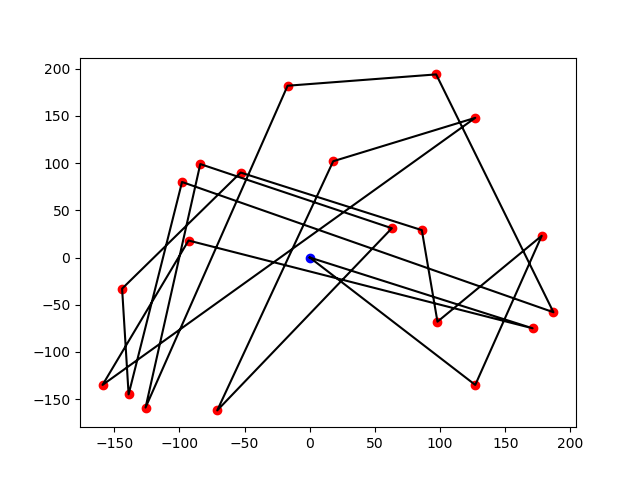
\includegraphics[scale=0.4]{test4_20_init.png}
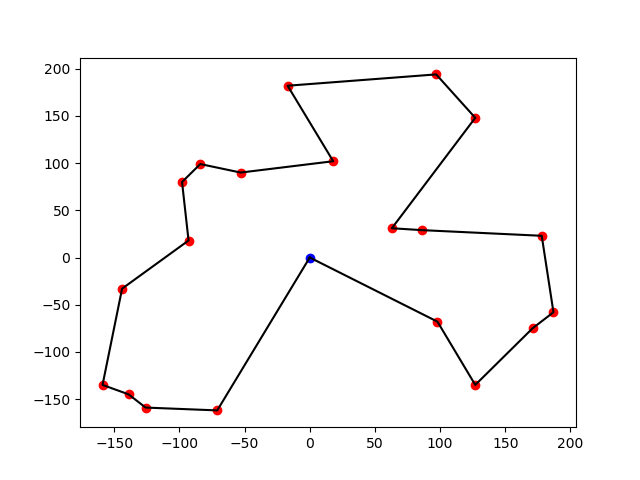
\includegraphics[scale=0.4]{test4_20_LKopt.png}

\caption{Exemple de fonctionnement de l'opérateur LK}
\label{LK}
\end{figure}

L'algorithme~\ref{algo:LK} décrit l'exécution de l'opérateur.

\begin{algorithm}
\DontPrintSemicolon % Some LaTeX compilers require you to use \dontprintsemicolon instead
\KwIn{Une tournée $r$ à améliorer}
\KwOut{Une permutation de $r$ ayant un meilleur coût que $r$}
$r_{next} \gets 2$-$opt(r) $\;
\While{$ r_{next} \neq r$} {
  $r \gets r_{next}$\;
  $r_{next} \gets 2$-$opt(r)$\;
}
\Return{$r$}\;
\caption{{\sc Lin-Kernighan} applique l'opérateur Lin-Kernighan}
\label{algo:LK}
\end{algorithm}

Lorsqu'il s'agit d'appliquer \emph{2-opt}, il est possible d'utiliser les méthodes de la section \ref{voisinage} pour explorer les voisinages.

\subsection{Algorithme d'optimisation utilisé}
L'algorithme d'optimisation que nous utilisons est un peu différent de l'heuristique A\&S précédente.
Pour diminuer le temps d'exécution, nous choisissons de diminuer le temps limite entre deux nouvelles solutions à $\frac{n}{3}$ secondes. 
Pour que l'exploration du voisinage des solutions soit plus efficace, nous décidons de passer les opérateurs \emph{EC} et \emph{CE} en mode $FI-RD$ (ce qui est généralement le cas dans les algorithmes d'optimisation).
Enfin, nous ajoutons une condition de \emph{Restart}, s'il n'y a pas eu d'améliorations depuis $n$ itérations.

L'algorithme~\ref{algo:HC} présente en rouge les changements effectués.

\begin{algorithm}
\DontPrintSemicolon % Some LaTeX compilers require you to use \dontprintsemicolon instead
\KwIn{Un ensemble de points I, les demandes des clients D, un triplet de flottants $(\lambda,\mu,\nu)$}
\KwOut{Une solution au problème I}
$Sol \gets CW(I,D,\lambda,\mu,\nu)$\;
$N \gets length(D)$\;
$nextSol \gets Sol$\;
\While {La dernière amélioration date de moins de \textcolor{red}{n/3 sec}} {
	$worstEdge \gets argmax_{(i,j)} b(i,j) $\;
	$nextSol \gets EC_{\textcolor{red}{FI-RD}}(worstEdge,I,D)$\;
	$nextSol \gets LK_{BI-O}(nextSol)$\;
	$nextSol \gets CE_{\textcolor{red}{FI-RD}}(worstEdge,I,D)$\;
	$nextSol \gets LK_{BI-O}(nextSol)$\;
	\If {$cost(Sol) > cost (nextSol)$} {
		$ Sol \gets nextSol$\;
	}
	\textcolor{red}{
	\If {Pas d'améliorations depuis $n$ itérations} {
		$nextSol \gets Sol$\;
	}
	}
	\If {Pas d'améliorations depuis $n$ itérations} {
		Changer de fonction de pénalisation en prenant un autre triplet $(\gamma_w,\gamma_c,\gamma_d)$\;
		Réinitialiser les pénalités des arêtes\;
	}
}
\Return{$Sol$}\;
\caption{{\sc $H_c$} calcule une solution du problème considéré}
\label{algo:HC}
\end{algorithm}

Nous pouvons à présent nous intéresser à l'extraction des connaissances des solutions initiales.

\section{Extraction de la connaissance}
Cette section s'intéresse à l'extraction de connaissance à partir de solutions initiales générées. 

\subsection{Quelle est la connaissance ?}
En observant quelques solutions obtenues avec CW, et application de l'opérateur LK, on remarque que plus la solution initiale est bonne et plus elle possède d'arêtes en commun avec la solution optimale. Ce résultat est illustré sur les figures~\ref{edges190115} à \ref{edges010101}, où les arêtes optimales sont vertes.

\begin{figure}
\begin{center}


  	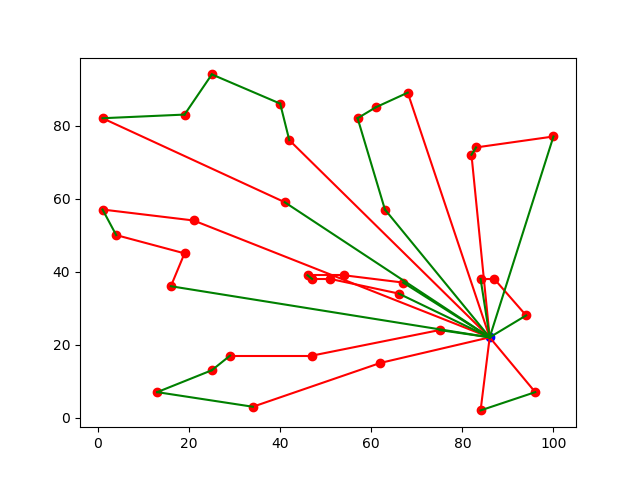
\includegraphics[scale=0.4]{edges190115.png}
	\caption{$CW(1.9,0.1,1.5)+LK$, $cost = 1041$, 19 arêtes optimales}
	\label{edges190115}
  
	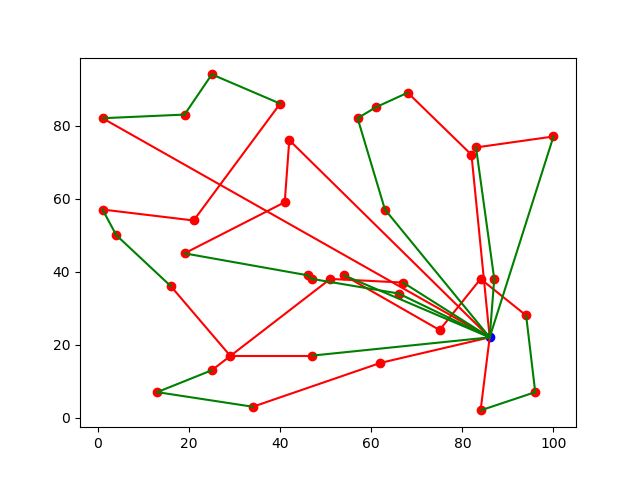
\includegraphics[scale=0.4]{edges101010.png}
	\caption{$CW(0.1,0.1,0.1)+LK$, $cost = 1170$, 19 arêtes optimales}
	\label{edges101010}

	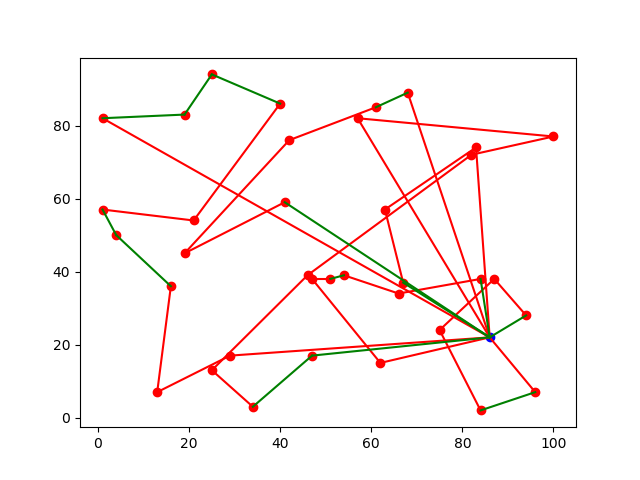
\includegraphics[scale=0.4]{edges010101.png}
	\caption{$CW(0.0,1.0,1.5)+LK$, $cost = 1600$, 11 arêtes optimales}
	\label{edges010101}	
	
\end{center}
\end{figure}

Il faudrait donc pouvoir déterminer à l'avance les arêtes optimales à partir des solutions initiales fournies par $CW+LK$.

\subsection{Protocole d'apprentissage}
Pour extraire cette connaissance, nous allons devoir créer un échantillon de solutions initiales, à partir duquel nous allons extraire une base d'apprentissage. Cette base va nous permettre d'extraire des arêtes.

\subsubsection{Génération de l'échantillon}
Puisque l'on ne peut pas prédire les paramètres $(\lambda,\mu,\nu)$ pour obtenir de bonnes solutions, nous allons devoir en générer un certain nombre :
\begin{itemize}
\item Soit on génère l'intégralité des solutions initiales possibles, en parcourant tous les triplets $(\lambda,\mu,\nu)$ (ie génération de 8820 solutions), pour obtenir l'échantillon;
\item Soit on tire $N$ triplets $(\lambda,\mu,\nu)$ aléatoirement, et les solutions obtenus constitueront notre échantillon. 
\end{itemize}

Les solutions qui constituent notre échantillon ne sont pas nécessairement toutes différentes.

\subsubsection{Construction de la base d'apprentissage}

\subsubsection{Extraction des arêtes}

\subsection{Résultats}



\section{Intégration de la connaissance} 

\subsection{Où intégrer la connaissance ?}

\subsection{Learning Heuristic}

\subsection{Résultats}

\bibliographystyle{plain}
\bibliography{biblio}

\end{document}